% !TeX root = ../main.tex

\chapter{绪论}
\label{chap:intro}

基于闪存的固态硬盘(SSD)正在数据中心中得到越来越广泛的应用。
与机械硬盘(HDD)相比,SSD的吞吐和访问延迟都有数量级的提升~\cite{chen2009understanding}。
特别地,由于内部存储介质不同,SSD的随机访问性能尤为出色。
因此,主流的云计算厂商,如Azure、AWS等,都提供了基于SSD的高性能存储服务~\cite{awsebs,azuredisks}。
专门针对固态硬盘进行优化的键值存储引擎RocksDB也得到了广泛的部署~\cite{cao2020characterizing,rocksdb,siying2021rocksdb}。

云闪存系统的服务质量往往是由吞吐、延迟等性能决定的。
对于云服务商而言,对于服务质量的保证是他们对租户的服务等级协议(SLA,Service Level Agreement)的一部分。
例如,AWS的io2 SSD服务,提供了500IOPS/GiB,最高达64KIOPS的吞吐~\cite{awsio2}。
近期的新存储服务,例如Azure Ultra Disk~\cite{azureultradisk},提供次毫秒级的延迟保证。
由于在分布式在线服务中,尾延迟受到了关注~\cite{dean2013tail},因此学术界也开始关注为SSD服务提供尾延迟保证~\cite{klimovic2017reflex}。

% 与此同时,为了解决数据中心资源利用率低的问题~\cite{kanev2015profiling},研究人员提出了资源池化(Resource Disaggregation)的方法~\cite{shan2018legoos,klimovic2016flash}。
% 通过将原本紧耦合的CPU、内存、硬盘等资源分别组织成独立的资源池,云服务商可以调度多租户共用物理资源,使有限的资源得到尽可能大的复用,避免浪费。
% 因此,资源池化在学术界和工业界都受到了广泛的关注。
% 目前,资源池化已经广泛地存在于云存储服务中。
% Azure Blob Storage~\cite{azureblob}、AWS S3~\cite{awss3}等对象存储服务
% 和Azure Disk Storage~\cite{azuredisks}、AWS Elastic Block Store~\cite{awsebs}等块存储服务
% 都提供了独立于计算服务的、多租户共享的存储抽象。

然而,想要在SSD上提供良好的SLA并不容易。
这是因为SSD的内在机制给服务质量带来了新的挑战——多租户间的性能隔离。
当多个租户共享同一块物理硬盘时,他们的访问性能不应相互影响。
这一保证在SSD上不易实现。
由于基于闪存的SSD的内在特性,共享同一块物理SSD的多个租户之一进行的写操作可能会触发SSD的垃圾回收、缓冲区清除等内部维护行为,这些行为将会影响其它租户的访问性能。
特别地,这一读写干扰~\cite{klimovic2017reflex}问题会使其它租户的访问尾延迟增加数倍。
对于追求快速响应的Web服务而言,这意味着其服务质量将受到较大的影响~\cite{dean2013tail}。
因此,追求低延迟的应用仍倾向于使用本地独占的SSD存储~\cite{awsvm,azurevm}。

\begin{figure}[h]
  \centering
  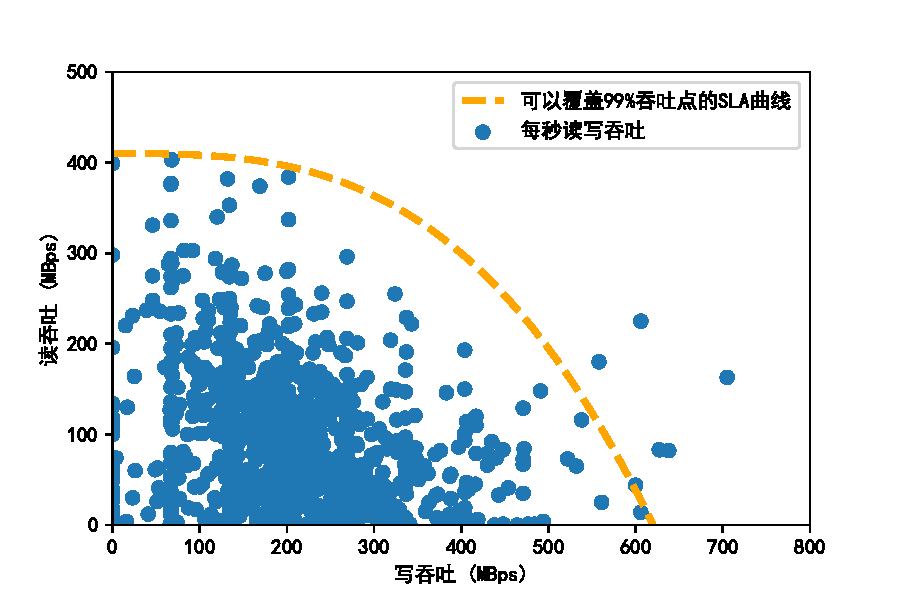
\includegraphics[width=0.8\textwidth]{thesis-intro-ycsb.pdf}
  \caption{
        YCSB负载A在RocksDB上运行时,每秒的读写吞吐没有固定的比例,且几乎不会同时达到最大的读和写吞吐,因此更适合用曲线描述其带宽需求。
      }
  \label{fig:intro}
\end{figure}

简单限制各个租户分享到的最大带宽的方式不能限制读写干扰,因此不能实现性能隔离。
并且,由于SSD的读写操作对磁盘的影响并不对称,需要同时考虑租户的读和写带宽。
事实上,租户在不同时间往往有不同的读写吞吐比例,他们的最大吞吐更适合用一条由不同读写带宽包围出的曲线表示。
\autoref{fig:intro}所示为~\citet{yadgar2021trace}采集的将YCSB负载A在RocksDB上运行得到的块请求记录,图中截取了其在10分钟每秒的读写吞吐。
由图可见,其读写吞吐在不同的比例之间变化,且几乎不会同时达到最大的读和写吞吐。

因此,本文使用\textit{SLA曲线}来描述服务质量。
具体来讲,SLA曲线表示的是在某个尾延迟要求下的最大读写带宽。
例如,\autoref{fig:intro}中的橙色虚线就可以作为以上YCSB负载的SLA曲线。
该曲线覆盖了99\%的读写吞吐,它基本代表了该负载对IO资源的需求。

针对以上问题,本研究搭建了一个具有多租户性能隔离功能的云闪存系统,该系统具有如下设计目标:
\textbf{1)高资源利用率}。
在云系统中,资源调度不再受限于“服务器”这一有限的单位。
本系统可以调度多租户共享同一物理硬盘上的存储空间和带宽,达到资源的高效利用;
\textbf{2)用户自定义SLA}。
在云闪存系统中,用户对存储资源的需求也不再受限于服务器上有限的资源。
本系统允许用户使用\textit{SLA曲线}定义其需要的读写带宽及达到该带宽时的尾延迟,系统会根据该定义为用户自动分配适合的存储硬盘。
\textbf{3)低尾延迟}。
本系统将各租户可保证的尾延迟作为存储性能隔离的评价指标。
通过减少或控制占用同一物理硬盘的各租户间的读写干扰,本系统可以降低各租户的尾延迟,从而实现有效的存储性能隔离。
\autoref{tab:cmp-ebs-insstore}中为本系统与目前主流云存储系统的对比。

\begin{table}[h]
  \centering
  \caption{本系统与常见云存储系统的对比}
  \label{tab:cmp-ebs-insstore}
  \begin{tabular}{cccc}
    \toprule
    \textbf{} & 高资源利用率 & 自定义SLA & 低尾延迟  \\
    \midrule
    传统池化存储系统 & \cmark & 部分 & \xmark  \\
    直连的闪存系统 & \xmark & \xmark & \cmark   \\
    \textbf{本系统} & \cmark & \cmark & \cmark  \\
    \bottomrule
  \end{tabular}
\end{table}

为了实现以上设计目标,本系统进行了如下设计。
首先,为了改善多租户读写干扰问题,本系统设计了无读写干扰的SSD阵列。
本系统提出\textit{分离的读写时间窗口},将对SSD的读写混合访问拆分为交替的纯读和批量写访问。
在纯读时间窗口中,本系统将所有写请求存于缓冲区中,从而获得无干扰的读性能;
纯写窗口中批量写入写请求,从而最大程度利用SSD的写带宽。
为了在纯写窗口中仍能服务读请求,本系统通过RAID~\cite{patterson1988case}或纠删码~\cite{huang2012erasure}等方式引入冗余。
通过协调不同硬盘中的时间窗口,使得所有数据总能被以无干扰的延迟被访问。

在此基础上,针对不同用户的不同SLA需求,本系统设计了基于SLA曲线的SSD资源分配算法。
本研究提出用SLA曲线定义用户的服务质量要求,并进一步定义了SLA曲线的加法、减法、包含等运算。
基于SLA曲线这一定义,本系统提出了一个多租户、多SSD数据分布的在线启发式算法。
该算法受向量装箱问题~\cite{panigrahy2011heuristics,hu2003operations}的启发,采用最佳适应算法,为系统中的租户提供了SLA保障,还得到了高效的资源利用率。
此外,本系统还实现了一个基于SLA曲线的IO请求调度器,它在运行时根据租户的实际吞吐,为每个租户提供SLA规定的吞吐和尾延迟保证。

本文的后续章节按如下方式组织:
第二章介绍本研究的动机——闪存资源池化系统中的多租户性能隔离问题,并介绍在保证SSD的服务质量方面的相关工作;
第三章介绍本研究所提出的系统设计,并详细介绍如何构建无读写干扰的冗余SSD阵列,以及基于背包问题的用户需求分配算法;
第四章介绍该系统的实现方式;
第五章通过大量实验证明了该系统的有效性;
第六章为本研究的总结。